En el presente documento se expone el desarrollo del Trabajo Terminal ``Sistema de recomendaciones basado en aprendizaje máquina y aplicación móvil conectada con emisores de señal Bluetooth Beacon (Sapphire)''  con número 2017-B034. Expone el análisis de las problemáticas que dieron origen a esta idea, así como la solución que fue propuesta y entorno a la cual se desarrolla actualmente el proyecto, teniéndose en cuenta el alcance del proyecto con respecto a los tiempos de ejecución y los riesgos que la realización de este conlleva.
\\ \par
Dentro de la propuesta de solución a los problemas identificados, se presenta la justificación a dicho trabajo y los objetivos que se desean cumplir.
Posteriormente, dentro del marco teórico se explican de forma más precisa ciertos subcampos, algoritmos y técnicas de las ciencias de la computación, así como los dispositivos y las bibliotecas que serán utilizadas.
\\ \par
En el apartado del análisis encontramos el análisis de factibilidad con el cual se pretende evaluar si se cuenta con la tecnología necesaria para el desarrollo del sistema y el costo total que este tendría. Así mismo, se analizan los requerimientos tanto funcionales como los no funcionales y de igual forma, son analizados y se priorizados los riesgos que se  localizan.
\\ \par
Finalmente, se muestran una serie de diagramas y modelos que explican de manera gráfica el comportamiento del sistema y la arquitectura de este.
\\ \par
Este documento va dirigido a toda la comunidad politécnica y externos a ésta a fin de proveer una nueva fuente de información que permita crear o innovar la manera en que se les proporciona la información publicitaria a los clientes dentro de un enfoque comercial.
\\ \par


Realizado por:\\
Castro Flores Marcela\\
Galindo García Adrián Eduardo\\
Murga Dionicio Rubén Adolfo 
\\ \par

Escuela Superior de Cómputo - Instituto Politécnico Nacional
\\ \par
%--------------------------------------------------
\section{Contexto}
En los últimos años, internet se ha poblado con miles de plataformas tales como: Amazon, Apple Music, Mercadolibre, Netflix, Twitter, Spotify, entre muchas otras, que incorporan millones de usuarios, los cuales generan infinidad de datos, mismos que a su vez han ocasionado la implementación y la gran popularidad de sistemas que permitan filtrar, priorizar y otorgar información relevante, mejor conocidos como sistemas de recomendaciones. Este tipo de sistemas realizan una búsqueda a través de un gran volumen de información generada dinámicamente para proporcionar contenidos y servicios personalizados, utilizando algoritmos que en su mayoría provienen del campo del aprendizaje máquina. El aprendizaje máquina es un subcampo de la inteligencia artificial que permite a las computadoras aprender de información y datos proporcionados sin programar explícitamente reglas a seguir. Por ejemplo, un sistema de recomendaciones podría ser utilizado en puntos de venta en línea para ofrecer a los clientes sugerencias sobre lo que les gustaría comprar, basándose en su historial de compra y/o búsqueda de productos.
\\ \par
%--------------------------------------------------
\section{Problemática}
Hoy en día, los sistemas de recomendaciones implementados en las tiendas departamentales se han limitado a otorgar beneficios por medio de ventas en línea y en monederos electrónicos, lo cual no tiene una rentabilidad directa con las ventas físicas, además de que, muchas de las recomendaciones que se ofrecen al público son generalizadas lo cual disminuye el interés de los clientes por los productos recomendados. Tomando esto en cuenta, a continuación en el cuadro \ref{table:comparacion}, se presenta una comparación entre los sistemas de venta en línea contra los sistemas de venta tradicional.
\FloatBarrier
\begin{table}[htb]
\setlength\extrarowheight{2pt} % for a bit of visual "breathing space"
\begin{tabularx}{\textwidth}{|C|C|}
\hline
\textbf{Sistemas de venta en línea} & \textbf{Sistemas de venta tradicional} \\\hline

El número de clientes a los cuales se puede dirigir un producto es mayor debido a que virtualmente el cliente tiene acceso a cada uno de ellos y puede filtrarlos para encontrar el de su preferencia.
& 
Se obtienen los productos con una satisfacción inmediata, es decir, no se tiene que esperar un determinado plazo de días para que el producto llegue al consumidor, por lo que tampoco se tiene que pagar un costo extra por envío.  
\\ \hline
\multicolumn{2}{|c|}{Ventajas} \\ \hline
Las recomendaciones que se le presentan al usuario son basadas en productos relacionados con los que se han visto o comprado con anterioridad,  por lo tanto son útiles y acertadas.
&

Se proporciona a los clientes un mejor asesoramiento sobre las especificaciones de los productos, ya que en las tiendas, el cliente puede preguntar lo que desee y tener una respuesta inmediata.
\\ \hline

Permite dar una retroalimentación sobre el producto por parte de los usuarios que compraron dicho producto.
&
El cliente puede visualizar, incluso hasta probar los productos que está por comprar.
\\ \hline

Por medio de un sitio Web, el cliente tiene acceso a cualquier hora del día para consultar y/o adquirir los diferentes productos propuestos.
&
Contrariamente a lo anterior, una tienda física funciona en un horario definido por lo cual las ventas se ven restringidas a dicha jornada del día. 
\\ \hline
\multicolumn{2}{|c|}{Limitantes} \\ \hline

Existen personas que no confían al 100\% en la compra de productos en plataformas en línea ya que temen que al proporcionar sus datos personales estos sean utilizados para otros fines.
&
Aún y cuando los empleados proporcionan atención al cliente, en ocasiones ofrecen mercancía fuera de su interés, lo cual llega a ser molesto.
\\ \hline

En ocasiones el comprador necesita visualizar y/o probar el producto antes de estar seguro de realizar su compra. 
&
No permite visualizar opiniones sobre el producto hechas por compradores anteriores. 
\\ \hline

\end{tabularx}
\caption{Comparación entre sistemas de venta en línea y sistemas de venta tradicional \cite{Sistemasventa}\cite{NextU}.}
\label{table:comparacion}
\end{table}
\FloatBarrier


Por otro lado, en años recientes se han creado también muchas aplicaciones que hacen uso de la geolocalización de los usuarios por medio de Internet o del Sistema de Posicionamiento Global (Global Positioning System, por sus siglas en inglés GPS), y su vez se ha dado el crecimiento de unos pequeños dispositivos conocidos como Beacons, los cuales emiten señales de corto alcance por medio de la tecnología Bluetooth de bajo consumo (Bluetooth Low Energy, por sus siglas en inglés BLE). Debido a su corto alcance (5 a 100 metros en promedio) resultan muy efectivos para dicha geolocalización en proximidad. Un claro ejemplo del uso de estos dispositivos está dentro del marketing de proximidad, tanto por la facilidad de puntos de referencia como por los anuncios de ofertas e información de productos que pueden proveer \cite{nicolas}. 


%--------------------------------------------------
\section{Estado del arte}

Se realizó una investigación para conocer si en la actualidad se han desarrollado aplicaciones similares tanto dentro como fuera del Instituto Politécnico Nacional (IPN). La búsqueda fue realizada tanto en el sitio oficial de la Escuela Superior de Cómputo (ESCOM) y en su biblioteca como en sitios externos a este, con el fin de conocer los trabajos terminales realizados previamente que fueron enfocados al desarrollo de un software similar o que de igual manera utilizaron Beacons para estos.
Para obtener una perspectiva teórica sobre los dispositivos que se plantean utilizar y que ya se han utilizado en las aplicaciones encontradas, podemos encontrar la definición de los Beacons en la sección Glosario de Términos.
\\ \par
Se explican los sistemas de recomendaciones que se han realizado con anterioridad, elaborados para un uso comercial dentro de tiendas departamentales y que a su vez, utilizan dichos dispositivos.De igual manera, se explica el funcionamiento de los Trabajos Terminales (TT) desarrollados dentro de la ESCOM que utilizan Beacons y de igual manera desarrollan sistemas de información. Cabe mencionar que los sistemas de ámbito comercial, se desarrollaron por parte de tiendas departamentales de gran renombre como lo es la tienda Macy's de Nueva York y San Francisco, el supermercado Carrefour, muy conocido por todo Europa, la tienda de ropa American Eagle Outfitters, entre otras, las cuales han obtenido grandes beneficios a partir del uso práctico de los Beacons.
\\ \par
\subsection{Tienda departamental Macy's}
Macy's es el primer minorista que ha hecho uso de los iBeacons de Apple desde el año 2013 a la actualidad, a partir de los cuales, envía diferentes tipos de alertas a los usuarios de iPhone con el fin de informarles acerca de las diferentes ofertas y productos que pueden ser de su interés y que claro, se encuentran a la venta en la tienda.
Este funcionamiento es realizado por medio de la aplicación conocida como "Shopkick", misma a la cual son redirigidos los compradores al ingresar a Macy's \cite{MACY'S1}. Esta aplicación que inició como una prueba en el año 2013, en las sucursales de Macy's Herald Square en Nueva York y en Union Square en San Francisco y  que se limitaba a hacer un ping a los iPhones de los clientes al momento en que ellos ingresaban a la tienda, se ha expandido hasta el año pasado en el Black Friday, durante la campaña "Walk in and Win", en el cual los clientes obtenían en la aplicación el típico juego de "rasca y gana" pero virtual y durante la jornada de compras alrededor de toda la tienda, ellos debían estar atentos pues podían adquirir grandes beneficios como tarjetas de regalo y reuniones con celebridades \cite{MACY'S2}.
\\ \par
La figura \ref{image:macysapp} muestra la interfaz de usuario que la aplicación de Macy's "Walk in and Win'' ofrecía a sus consumidores.
\FloatBarrier
\begin{figure}[htbp!]
		\centering
			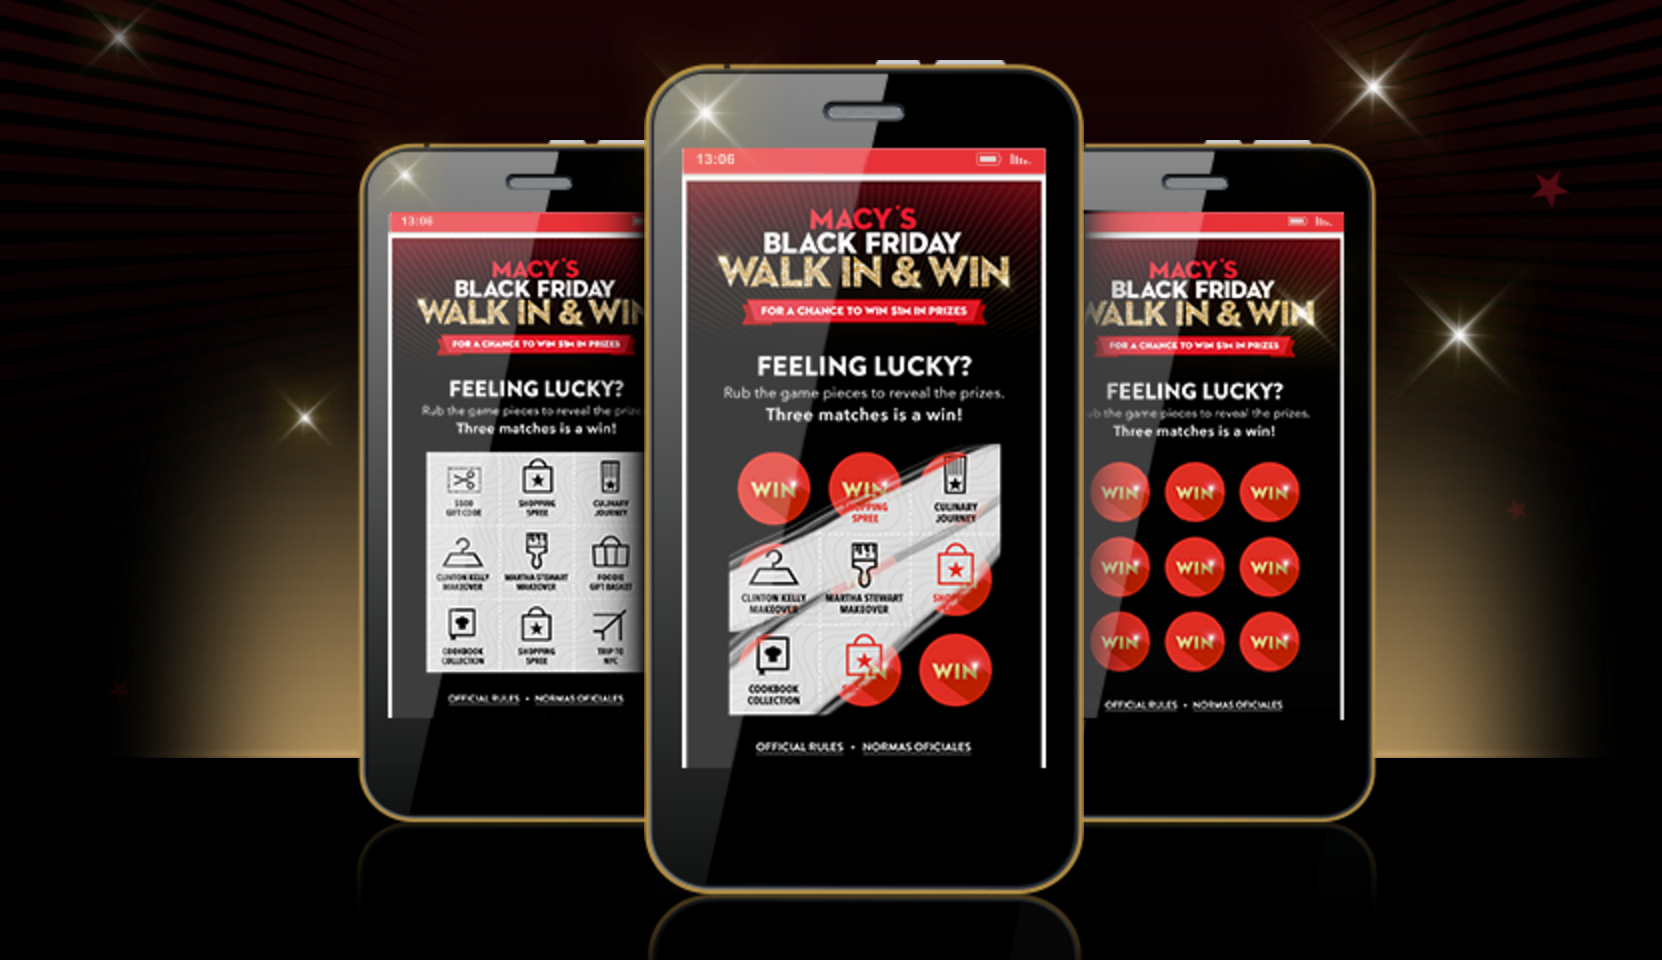
\includegraphics[width=.45 \textwidth]{imagenes/walkinandwin}
		\caption{Aplicación de Macy's "Walk in and Win"  \cite{MACY'S3}.}
		\label{image:macysapp}
\end{figure}
\FloatBarrier

\subsection{Supermercado Carrefour}
En el 2015, el supermercado Carrefour instaló 600 Beacons BLE  en sus 28 hipermercados en Rumania para guíar a los compradores a lo largo de toda la tienda y al mismo tiempo, estos recibían promociones y ofertas tanto en sus dispositivos móviles como en las tablets incorporadas al manubrio de los carritos de supermercado. Esta empresa hacía uso de la tecnología Beacon marca Onyx Beacon, misma que se ha encargado de instalar dichos dispositivos a lo largo de autobuses y trolebuses en Bucharest a fin de guiar a los pasajeros con discapacidades visuales.
El uso de la aplicación era simple y consistía en indicar la ruta óptima por toda la tienda al cliente, con el fin de que obtuviera todos los artículos que previamente había seleccionado de cada uno de los departamentos disponibles del supermercado. A manera en la que el cliente avanzaba por toda la tienda, este recibía diferentes promociones y notificaciones sobre los productos del departamento en el que se hallaba \cite{NFC}.
\\ \par
La figura \ref{image:smartCarrefour} muestra uno de los carritos del supermercado Carrefour a los cuáles se les implantaron las tablets con la aplicación "Smart Shopping" para que el cliente realizara su recorrido dentro de la tienda mientras obtenía a su paso por los diferentes departamentos, promociones y descuentos.

\FloatBarrier
\begin{figure}[htbp!]
		\centering
			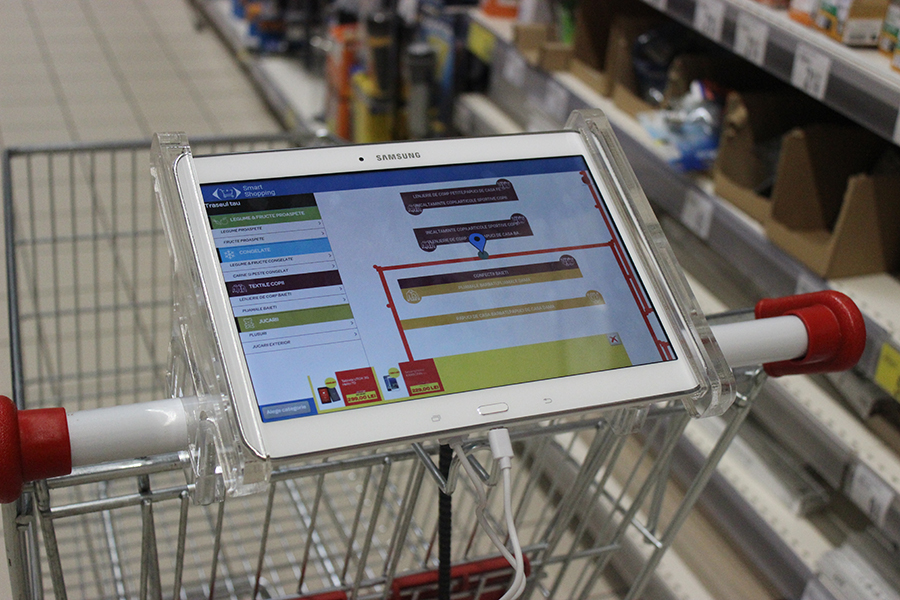
\includegraphics[width=.45 \textwidth]{imagenes/samsung}
		\caption{Aplicacíón "Smart Shopping" de Carrefour trabajando sobre una tablet "Samsung"  \cite{OnyxBeacon}.}
		\label{image:smartCarrefour}
\end{figure}
\FloatBarrier
\subsection{Tienda de ropa American Eagle Outfitters}
En el caso de la tienda de ropa American Eagle, tomaron en cuenta que los clientes que entran a los probadores son más propensos a adquirir una prenda de ropa por lo cual, en el año 2014, haciendo uso de la misma aplicación que la tienda Macy's, instaló en 100 de las 929 tiendas de la marca, Beacons en los probadores, mediante los cuales se enviaban ofertas a los usuarios. Para ello, fue importante encontrar que aquellos clientes que recibían una oferta, estaban más predispuestos a probarse otra prenda a diferencia de aquellos que no lo hacían \cite{AEO}.
\\ \par
En la figura \ref{image:americanEagle} se presenta una de las sucursales de la tienda de ropa American Eagle Outfitters que instaló los dispositivos Beacons dentro de los probadores de los clientes con el fin de enviarles diferentes descuentos y de este modo, promover el aumento en las ventas de la ropa.
\FloatBarrier
\begin{figure}[htbp!]
		\centering
			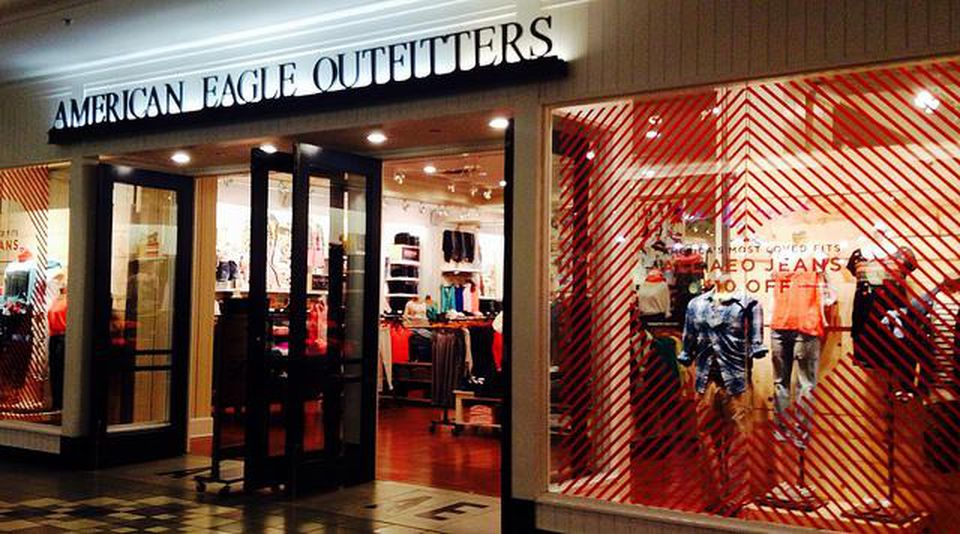
\includegraphics[width=.45 \textwidth]{imagenes/AEO}
		\caption{Tienda de ropa American Eagle Outfitters \cite{Forbes}.}
		\label{image:americanEagle}
\end{figure}
\FloatBarrier
\subsection{Aplicación makeitapp}
Finalmente y una de las aplicaciones que nos pareció muy importante de considerar fue la aplicación makeitapp debido a que esta empresa permite realizar todo el desarrollo de una app personalizada haciendo uso de los Beacons y a su vez, provee de un panel de control al administrador. A primera vista esta aplicación tiene cierta similitud con el TT propuesto ya que realiza el envío de notificaciones que sugieren productos y servicios personalizados, sin embargo, la diferencia que este sistema presenta es que no ofrece al cliente la asistencia directa por parte de un vendedor cuando él/ella ha ingresado a la tienda departamental \cite{makeitapp}.
\\ \par
Ya que se han descrito con mayor profundidad lo que los sistemas anteriores realizan, se muestra a continuación una comparación entre estos. El cuadro \ref{table:sistemascomercialesapps} se enfoca principalmente en las características que cada uno de los sistemas implementa mismo que a su vez se compara con las características del sistema a desarrollar.

\FloatBarrier
\begin{table}[htb]
\setlength\extrarowheight{2pt} % for a bit of visual "breathing space"
\begin{tabularx}{\textwidth}{|C|C|C|C|C|C|}
\hline
\textbf{Característica/Sistema} & \textbf{Tienda departamental Macy's} & \textbf{Supermercado Carrefour} & \textbf{Tienda de ropa American Eagle Outfitters} & \textbf{makeitapp} & \textbf{Sapphire} \\\hline
Uso de Beacons & Sí & Sí & Sí & Sí & Sí \\ \hline
Aplicación móvil & Sí & Sí & Sí & Sí & Sí \\ \hline
Atención personalizada & No & No & No & No & Sí \\ \hline
Plataforma Web (Panel de control) & Sí & Sí & Sí & Sí & Sí \\ \hline
Ludificación & Sí & Sí & Sí & Sí & Sí \\ \hline
Recomendaciones personalizadas & No & No & No & No & Sí \\ \hline
\end{tabularx}
\caption{Comparación entre sistemas desarrollados para tiendas comerciales.}
\label{table:sistemascomercialesapps}
\end{table}
\FloatBarrier
Ahora proseguimos con el análisis de los TT's realizados en la ESCOM entre los cuales obtuvimos 2 que son los que más se asemejan al tema que se busca desarrollar.
%\subsection{TT 2016-A087 Desarrollo de un sistema de recomendación de productos usando herramientas de Big Data.}
%A.[16]
\\ \par
\subsection{TT 2015-A056 API para el desarrollo de sistemas de recomendación.}
Lo que este Trabajo Terminal proponía era la realización de una Interfaz de Aplicación de Programación (Application Programming Interface, por sus siglas en inglés API) que permitía desarrollar diferentes sistemas de recomendación con el fin de brindar diferentes funciones de abstracción, clasificación y análisis de los datos recopilados. Se centraban en el caso de estudio de un restaurante con diferentes platillos en una zona geográfica en particular \cite{API}.
\\ \par
\subsection{TT 2010-0063 Trabajo Terminal Sistema generador de recomendaciones para una tienda en-línea de videojuegos.}
Este trabajo consistió en una plataforma Web de información, enfocada a la venta de artículos de entretenimiento haciendo uso de un sistema de recomendaciones con el fin de mejorar las compras de sus usuarios \cite{TT3}.
\\ \par
Posteriormente, en el cuadro \ref{table:comparaciontrabajosterminales} se muestra la comparación entre el TT propuesto y aquellos que se han realizado con anterioridad dentro de la ESCOM.

\FloatBarrier
\begin{table}[htb]
\setlength\extrarowheight{2pt} % for a bit of visual "breathing space"
\begin{tabularx}{\textwidth}{|C|C|C|C|}
\hline
\textbf{Característica/Sistema} & \textbf{TT 2015-A056} & \textbf{TT 2010-0063} &  \textbf{Sapphire} \\\hline
Uso de Beacons & No & No & Sí  \\ \hline
Aplicación móvil & Sí & No & Sí \\ \hline
Atención personalizada  & No & No & Sí \\ \hline
Plataforma Web (Panel de control) & Sí & Sí & Sí \\ \hline
Ludificación& No & No & Sí \\ \hline
Recomendaciones personalizadas& Sí & Sí & Sí \\ \hline
\end{tabularx}
\caption{Comparación entre Trabajos Terminales de ESCOM.}
\label{table:comparaciontrabajosterminales}
\end{table}
\FloatBarrier

%--------------------------------------------------
\section{Solución propuesta}

Considerando todo lo anterior, proponemos como proyecto de titulación el desarrollo de un sistema compuesto por múltiples subsistemas que permitan atacar algunas de las limitantes de los sistemas de venta tradicional, los cuales son: 

\begin{itemize}
\item Un módulo de gestión, procesamiento  y proveedor de datos de Retail
que funciona como interfaz de conexión con dos módulos basados en aprendizaje máquina el cual haciendo uso de la información relacionada con las compras anteriormente registradas, las preferencias y características del usuario formulará una serie de recomendaciones de productos, las cuales se presentarán por medio de una aplicación móvil al usuario final. 
Por otro lado, sirve como servicios de Transferencia de Estado Representacional (Representational State Transfer, por sus siglas en inglés REST) para la gestión de datos del sistema. 


\item Se propone una aplicación móvil dirigida hacia los clientes en la cual podrán recibir sugerencias en formato de alertas basadas en las preferencias del usuario y recompensas por usar la aplicación, formadas a partir del sistema de recomendaciones anteriormente mencionado.

\item Por otro lado, una aplicación hecha específicamente para vendedores, mediante la cual se les proveerá una lista de los clientes dentro de la tienda y se mantendrán las ubicaciones de los Beacons actualizadas; dichos vendedores tendrán la posibilidad de seleccionar un cliente y visualizar productos que podrían ofrecerles personalmente; esto será posible si y sólo si el cliente establece en sus configuraciones ser visible por los vendedores o si solicita atención. Cabe mencionar que de igual manera que en la aplicación del cliente, los productos sugeridos que se le muestren al vendedor para cada uno de los clientes serán obtenidos del sistema de recomendaciones.

\item Finalmente, el último módulo considerado es una plataforma Web, la cual fungirá como un panel de administración y herramienta de gestión de información en la que se podrán administrar usuarios, anuncios, promociones, establecimientos, además de ajustar los parámetros del sistema de recomendaciones para mejorar la precisión de las predicciones. 
\end{itemize}

Es importante mencionar que para el desarrollo de la comunicación de la aplicación móvil del cliente se hará uso del Kit de Desarrollo de Software (Software Development Kit, por sus siglas en inglés SDK) de proximidad de Estimote para establecer una comunicación con los Beacons, mismos que nos proporcionarán la ubicación en la que un usuario se estará posicionando dentro de la tienda departamental \cite{google}. 
\\

Estos sensores serán divididos por departamentos dentro de la tienda y así mismo, se desarrollará un módulo generador de registros artificiales que nos permitirá simular una gran cantidad de datos e ingresarlos al subsistema de recomendaciones para poder verificar la efectividad del mismo.
%, y a su vez, se tiene contemplado verificar el tiempo que un usuario ha permanecido dentro del rango de la emisión de señal del Beacon para evitar la saturación de alertas al usuario. También %

%--------------------------------------------------
\section{Justificación}
Según datos presentados por el Instituto Nacional de Estadística y Geografía (INEGI) quiénes respecto a lo publicado en el informe “Estadísticas a propósito del día mundial de internet (17 de mayo)” con fecha del 15 de mayo del 2017 informan que el 59.5\% de la población de seis o más años de edad en México se declaró usuario de Internet, mientras que el otro 40.5\% no lo usan y a su vez de ese 59.5\%, el 96.0\% hace uso del mismo de 1 a 7 días de la semana, siendo el otro 4\% la población que no lo utiliza en lo absoluto. Si bien las transacciones electrónicas (compras o pagos vía Internet) no son actividades recurrentes entre los internautas mexicanos, se observa un crecimiento respecto a resultados anteriores, pasando del 12.8\% en el 2015 al 14.7\% en el 2016. Este mismo informe hace mención de más datos relevantes como que el 73.6\% de la población de seis años o más cuenta con un dispositivo móvil y el otro 26.4\% hace referencia a los menores de 6 años que no hacen uso de dicho dispositivo. Asímismo se menciona que tres de cada cuatro de estos usuarios (76.0\%) cuentan con un teléfono inteligente (Smartphone), lo cual significa que este tiene acceso a internet y por lo tanto, el otro 24\% no cuentan con un dicho teléfono celular. Sin embargo sólo el 89\% de los usuarios con un celular inteligente se conectan a internet y el otro 11\% no realizan dicha acción \cite{estadistica}.
\\ \par
Por otra parte, debemos considerar los indicadores que las empresas comerciales al por menor (las cuales incluyen a las tiendas de autoservicio y departamentales) están reflejando en estos últimos meses, esto con el fin de conocer los ingresos reales que se están generando por el suministro de bienes y servicios ya que este será el sector al que estaríamos beneficiando; el comunicado de prensa número 296/17 de la INEGI informa que a tasa anual, los ingresos por suministro de bienes y servicios aumentaron 3.4\% mientras que las remuneraciones medias reales se redujeron (-)0.2\% y el personal ocupado (-)0.1\% durante el quinto mes del 2017, esto respecto al mismo mes de un año antes  \cite{comunicado}.
\\ \par

Los datos presentados anteriormente son importantes para la realización de este proyecto, debido a que este está enfocado a usuarios que cuentan con un dispositivo móvil y que a su vez tienen acceso a una conexión de Internet o a un plan de datos móviles pues deberán obtener la aplicación móvil de nuestro sistema por medio de la cual obtendrán las promociones y los artículos sugeridos, así mismo, es necesario que los clientes cuenten con un Smartphone pues estos son los que tienen una conexión Bluetooth que será la que permitirá realizar la comunicación entre el Beacon y el celular que nos permitirá saber la posición en la que la persona se encuentre.
\\ \par
Una de las múltiples ventajas que este trabajo terminal posee respecto a proyectos que se han desarrollado en el mercado últimamente, será la gran reducción de papel que se obtendrá a partir de la eliminación de folletos promocionales que se reparten comúnmente dentro de las tiendas departamentales. En un informe de la Universidad Tecnológica de Monterrey se menciona que, en México, se talan medio millón de árboles diariamente con el fin de obtener su pulpa virgen para la producción del papel, si se reciclará ese papel se ahorrarían 28 mil litros de agua y 17 árboles. De igual manera el Instituto Nacional de Ecología declara que México ocupa el tercer sitio en índices anuales de deforestación y un cálculo aproximado de este desperdicio es de  \cite{TecMty}:
\\ \par
Medida de 1 hoja con norma del Instituto Alemán de Normalización (Deutsches Institut für Normung, por sus siglas en alemán DIN)-A4: $297 mm \times 210 mm = 62370 mm^2 = 0,062 m^2$ 
\\
1 hoja pesa $80\frac{g}{m^2} \times 0,062m^2 = 4,8 g$\\
500 hojas pesarán $500 g \times 4.8 g = 2.400 g = 2.4 kg$
\\ \par
En adición a las ventajas del sistema es importante recalcar que existen sistemas de recomendación en múltiples plataformas como Amazon y MercadoLibre, pero ninguna de ellas te permite tener un contacto directo con el producto de una manera en la que uno como comprador tome la decisión más completa respecto a adquirir o no el artículo.
\\ \par
Por otra parte, se pretende aplicar en el proyecto el término “Gamification/Ludificación” mismo que es utilizado para referirse a brindar ciertas recompensas a un usuario a cambio de que él, en este caso, se registre en nuestra aplicación. Está actividad no ha sido implementada a la par del uso de los Beacons, si bien el marketing de proximidad permite enviar promociones a todo aquel que se encuentre dentro del radio de emisión de la señal Bluetooth, no envía sugerencias personalizadas, lo cual implica una característica sobresaliente sobre los sistemas ya existentes.
\\ \par
Por lo planteado en este documento, consideramos que esta es una propuesta valiosa como tema de titulación, para el cual, se utilizarán los conocimientos adquiridos en la carrera de Ing. en Sistemas Computacionales de las unidades de aprendizaje: Redes Neuronales, Desarrollo de Aplicaciones Móviles, Sistemas Web, además de los siguientes cursos y libros: \\

\begin{itemize}
\item Machine Learning, Stanford, Andrew Ng.  \cite{Andrew}.
\item Deep Learning A-Z: Hands-On Artificial Neural Networks \cite{eremenko}.
\item Machine Learning, Tom M. Mitchell  \cite{mitchell}.
\end{itemize}


%--------------------------------------------------
\section{Objetivos}

% - - - - - - - - - - - - - - - - - - - - - - - - -
\subsection{Objetivo general}
Diseñar e implementar un sistema de recomendaciones basado en aprendizaje máquina que funcione como el núcleo de un conjunto de aplicaciones móviles y una plataforma Web a fin de generar recomendaciones de productos y/o servicios de forma personalizada a clientes de una tienda departamental.
\\ \par
% - - - - - - - - - - - - - - - - - - - - - - - - -
\subsection{Objetivos específicos}
\begin{enumerate}[1.]
    \item Desarrollar el prototipo de una aplicación móvil para clientes en la cual recibirán además de las recomendaciones, anuncios, promociones y notificaciones al encontrarse dentro de la tienda departamental y estar dentro del rango de un Beacon.
    \item Crear un módulo encargado de generar registros artificiales que nos ayudarán a simular datos con los cuales podremos entrenar y poner a prueba las recomendaciones que el sistema produzca. 
    \item Desarrollar el prototipo de una aplicación móvil para los vendedores de una tienda departamental, con la que puedan dar una atención personalizada a los clientes ofreciendo recomendaciones de productos que sean de su interés o simplemente asesorar su decisión de compra. 
    \item Realizar el desarrollo del prototipo de una plataforma en línea para que los administradores de la tienda departamental puedan gestionar anuncios y promociones, además de ver gráficas sobre las características del mercado que se tiene.
    \item Implementar el SDK de proximidad de Estimote para comunicar a los Beacons con las aplicaciones móviles y conocer la ubicación del usuario con el objetivo de dar recomendaciones personalizadas dependiendo de la tienda/departamento donde se encuentre.
    \item Desarrollar un prototipo de un servidor de servicios REST para realizar las operaciones de lectura y escritura sobre el repositorio de datos y proveer de recomendaciones a las diferentes aplicaciones móviles. 
\end{enumerate}
%--------------------------------------------------
\section{Metodología}
La metodología seleccionada y la que el equipo considera como la más acertada para el desarrollo de este proyecto es el “Prototipado Evolutivo”, mismo que se caracteriza por permitir la construcción de un prototipo inicial al cual se le irán añadiendo diferentes componentes a medida que el proyecto avanza. Esta metodología  es funcional en escenarios en los cuales no se conocen por completo los requerimientos, provee al equipo con ventajas como la flexibilidad en los mismos y entregas rápidas de productos funcionales.
\\ \par
Se pretende para cada uno de los prototipos previstos, realizar las etapas de análisis, diseño y pruebas, mismos que se irán actualizando con cada nuevo ciclo como se muestra en la figura \ref{image:metodologiaprototipado} de la metodología y cada nuevo prototipo realizado. Dichos prototipos continuarán indefinidamente hasta que las expectativas del cliente, el objetivo general y los objetivos específicos sean cubiertos de una manera satisfactoria. 

\FloatBarrier
\begin{figure}[htbp!]
		\centering
			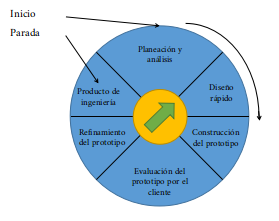
\includegraphics[width=.45 \textwidth]{imagenes/PE}
		\caption{Metodología de Prototipado Evolutivo \cite{Zachman}. }
		\label{image:metodologiaprototipado}
\end{figure}
\FloatBarrier

%--------------------------------------------------
\section{Beneficios esperados}
Como se ha explicado anteriormente, existen sistemas que han sido implementados en diferentes países, sin embargo, es importante recalcar que ninguno de ellos ha sido implementado ni probado en México, por otro lado, el uso y las funciones que los Beacons ofrecen, permiten romper la barrera que existe entre la tecnología y el mundo real. Es por eso que una de las principales metas a realizar es impulsar el uso de esta, así se implementan sistemas probados en países con un desarrollo tecnológico superior, lo que impulsa al desarrollo en el país y de esta forma, como ya se explicó en la justificación, se disminuyen las cantidades de residuos generados por folletos y otras propagandas distribuidas en las tiendas.
\\ \par
%--------------------------------------------------
\section{Alcance}
La implementación de un sistema que permita generar recomendaciones por medio de un esquema de aprendizaje máquina. Dicho sistema debe funcionar sobre aplicaciones móviles y una plataforma Web. La finalidad es generar recomendaciones de productos y/o servicios de forma personalizada a clientes de una tienda departamental.
\\ \par
%--------------------------------------------------
\newpage
\section{Limitantes}
Entre las principales limitantes a las que el sistema a desarrollar se enfrenta son: \\
\begin{itemize}
    \item Si la persona o el negocio no cuenta con servicio de Internet, no existe la comunicación entre los módulos por lo tanto es imposible el envío de recomendaciones a los clientes.
    \item Debido a los nuevos filtros de seguridad que Facebook ha impuesto, solo nos es posible obtener los datos básicos de un usuario como lo son su nombre, foto de perfil y su correo electrónico, por tal motivo, si dicho usuario no entra a la sección de "Gustos" para marcar las categorías que se relacionen con sus gustos, este no podrá ser clasificado dentro de una categoría y no podrá recibir recomendaciones acertadas.
    \item El tiempo de recolección de datos puede abarcar más tiempo de lo esperado debido a que cada usuario tiene un manejo diferente de la información dentro de sus redes sociales.
    \item Debido a no contar con datos reales con los cuales desarrollar este proyecto se desarrolló un generador de registros artificiales para generar datos de prueba. Esto ocasionó que algunos de los productos cuenten con imágenes repetidas, categorias y/o departamentos aleatorios.
    \item La SDK de Estimote se encuentra en constante actualización (al momento de iniciar el trabajo terminal se encontraba en pruebas beta), por esta razón, pueden ocurrir ciertos fallos o recargas en la pantalla de las aplicaciones móviles, especialmente en la creación de las zonas de proximidad las cuales requieren del Bluetooth del dispositivo.
    \item La realización de pruebas en dispositivos tales como Huawei P20, Xperia XA Ultra, Samsung Galaxy A5 y Xiaomi Redmi 4, nos permitió visualizar ciertos fallos ocurridos en únicamente algunos dispositivos. Por dicha razón, es importante considerar que dependiendo el hardware en el cual se hayan instalado las aplicaciones móviles, pueden ocurrir fallos referidos a la utilización del Bluetooth o las API's implementadas.
\end{itemize}
